\subsection{Trip Planning}
\label{app:trip}

\begin{figure}[htbp]
    \centering
    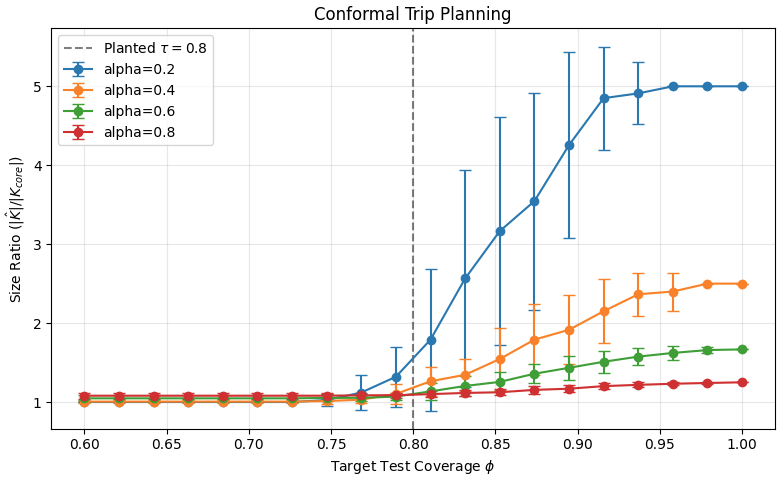
\includegraphics[width=0.6\linewidth]{images/tripplanning_conf.png} % Replace with your actual filename
    \caption{Trip Planning simulation with planted core probability $\tau=0.8$. The x-axis is the conformal guarantee $\phi$, and the y-axis represents the ratio of selected vertices to the optimal core size. }
    \label{fig:trip_planning}
\end{figure}

We next investigate a structured recommendation scenario where the goal is to recommend a bundle of activities (e.g., a vacation itinerary). We simulate a domain with $R=5$ distinct types of activities (e.g., dining, museums, hiking). For each type $r$, there is a set $A_r$ of available activities with $|A_r| = 10$. Within each type, we designate a "core" subset $A^*_r$ representing high-probability options, where $|A^*_r| = \alpha |A_r|$ for a density parameter $\alpha \in [0,1]$. The total vertex set is the union of all $A_r$. We generate hyperedges (itineraries) by selecting exactly one activity from each type. The generation process follows a planted model: For each type $r$ independently, the activity is drawn uniformly from the core $A^*_r$ with probability $p$, and uniformly from the complement $A_r \setminus A^*_r$ with probability $1-p$. The parameter $p$ is calibrated such that $p^R = \tau$, meaning that a "pure core" itinerary (composed entirely of core activities) occurs with probability $\tau$. In this setting, the ideal conformal set for mass $\tau$ is exactly the union of the core subsets, having a total size of $\sum |A^*_r| = \alpha \cdot |A_r| \cdot R$.

We fix the planted core probability $\tau = 0.8$ and vary the core density $\alpha \in \{0.2, 0.4, 0.6, 0.8\}$.  As before we generate $100$ training samples $\{Y_j\}_{j=1}^{T/2}$ and run the algorithm in Section~\ref{sec:mon} to obtain a nested sequence of subgraphs. For each conformal parameter $\phi$, we find the smallest subgraph achieving coverage $\phi$ on $100$ held out samples $\{Y_j\}_{j=T/2+1}^{T}$. (In other words, $T = 200$ in the algorithm in Section~\ref{sec:fixed_optimal}.) We plot the ratio of the number of vertices in the subgraph to the size of the ground-truth core, as a function of $\phi$ in Figure~\ref{fig:trip_planning}. A ratio of $1.0$ implies perfect recovery of the core.

The results highlight two key findings.  First, for all values of $\alpha$, the ratio remains strictly at $1.0$ as long as the target coverage $\phi$ is at most $0.75$, close to the true core probability $\tau$. This confirms that the LP rounding scheme correctly prioritizes the high-density core structure.  Second, we observe a sharp ``knee'' in the performance curves around $\phi = 0.8$. To satisfy a coverage request $\phi > 0.8$, the algorithm is forced to include hyperedges that contain non-core activities. Capturing this marginal probability mass requires adding a large number of new vertices, causing the ratio to rise sharply.   
